\documentclass[8pt,a5paper]{acm_proc_article-sp}
% fix umlauts
\usepackage[ngerman]{babel}
\usepackage[utf8]{inputenc} 
\usepackage[T1]{fontenc}  % Times new Roman
\usepackage{mathptmx}
\usepackage[]{blindtext}
\usepackage[a5paper, left=1.70cm, right=1.20cm, top=1.30cm, bottom=1.40cm]{geometry}
\usepackage{epstopdf}
% balance columns. original from acm doesn't work
\usepackage{balance}
% colors
\usepackage[compact]{titlesec}
\usepackage{natbib}
\titlespacing{\section}{0pt}{*0.7}{*0.5}

\usepackage[nolist]{acronym}
 
\usepackage[usenames,dvipsnames]{xcolor}
% automatic crosslinks
\usepackage[colorlinks=true,citecolor=black,linkcolor=black,filecolor=black,urlcolor=black,pagebackref=true]{hyperref}
\hypersetup{colorlinks=true,citecolor=black,linkcolor=black,filecolor=black,urlcolor=black,pagebackref=true}
%glossaries
%\usepackage{makeidx}
%\makeindex
%\usepackage[nomain]{glossaries}
%\makeglossaries
%\makeindex

\newcommand{\glspl}[1]{{#1}}

% http://en.wikibooks.org/wiki/LaTeX/Glossary
% http://mirror.informatik.uni-mannheim.de/pub/mirrors/tex-archive/macros/latex/contrib/glossaries/glossariesbegin.pdf

% Definitionsliste
\newcommand{\defitem}[1]{\item[#1]\phantomsection\label{#1}\hfill\\} 
\newcommand{\defref}[1]{\hyperref[#1]{#1}} 
\newcommand{\rem}[1]{}
% Marking colors
\definecolor{todo}{rgb}{1,0.2,0.2}
\definecolor{reconsider}{rgb}{0.6,0.6,0.3}
\newcommand{\todo}[1]{{\color{todo} #1}}
\newcommand{\reconsider}[1]{{\color{reconsider} #1}}



\graphicspath{{img/}{./}}
\usepackage{graphicx}
\title{PoSDBoS - Portable System to Detect Driver Drowsiness with
Body Sensors. \titlenote{ \scriptsize 
  \flushleft Betreuer Hochschule:  \ \ Prof. Dr. Martinez\\ 
  \qquad \qquad \qquad \qquad \quad \ \  Hochschule Reutlingen\\ 
  \qquad \quad \quad \quad \qquad \qquad \ \ Natividad.Martinez@Reutlingen-\\
  \qquad \qquad \qquad \qquad \quad \ \ University.de \\
  \includegraphics[width=1.8cm]{iot_hs_rt} \ \ \quad Master Project IoT 2016\\
  \ \ \\
  31. Juli 2016, Hochschule Reutlingen\\ 
  \copyright  ~ 2016 Paul Pasler}}


\numberofauthors{3}
\author{
	\alignauthor
	  \center
		\aufnt{Paul Pasler}\\
          \affaddr{Reutlingen University}\\
        \textbf{\textsf{Paul.Pasler@Student.Reutlingen-University.DE}}
}

\newcommand{\threadingSequence}{}
\newcommand{\docwidth}{11cm}

\begin{document}
\begin{acronym}
\acro{FAS}{Fahrerassistenzsystem}
\acro{FASs}{Fahrerassistenzsysteme}
\acro{ME}{Müdigkeitserkennung}
\acro{MESs}{Müdigkeitserkennungssysteme}
\acro{ADAS}{Advanced Driver Assistance System}
\acro{ADASs}{Advanced Driver Assistance Systems}
\acro{bspw}{beispielsweise}
\acro{RTU}{Reutlingen University}
\acro{BS}{Körpersensoren}
\end{acronym}



\maketitle
\sloppypar{
\begin{abstract}
\acl{FASs} sind aus modernen Fahrzeugen nicht mehr wegzudenken. \acl{ME} hilft Sekundenschlaf oder müdigkeitsbedingte Unachtsamkeit zu vermeiden und verhindert somit schwere Unfälle. Systeme mit \acl{BS} zeigen in verschiedenen Studien sehr genau Ergebnisse und erkennen Müdigkeit frühzeitiger als andere Ansätze. In der vorgelegten Arbeit wurde ein solches System mit einem Elektroenzephalogramm (EEG) umgesetzt und getestet. Hierfür wurden Testdaten aufgenommen, verarbeitet und mit einem künstlichen Neuronalen Netz klassifiziert, sodass der aktuelle Status des Fahrers "`Wach"' oder "`Müde"' unterschieden werden kann.
\end{abstract}

\keywords{
\acl{FAS}, \acl{ME}, Elektroenzephalogramm, Signalverarbeitung, Machine Learning, Neuronales Netz
}

\category{A.0}{ACM}{
Experimentation
}


\section{Einleitung}
\label{chap:intro}

\acl{FASs} sind innerhalb weniger Jahren von der Oberklasse in die Mittel- und Kleinwagenklasse vorgedrungen. Die Unternehmensberatung Strategy Analytics schätzt, dass in den nächsten Jahren sechs mal soviele \acl{FASs} verbaut werden als heute \cite{strategy_analytics}. Sie bieten dem Fahrer erhöhten Komfort (bspw. Tempomat) oder erhöhen die Sicherheit (bspw. Notbremsassistent). Laut der Boston Consulting Group, könnte der flächendeckende Einsatz von \acl{FASs} die Unfallrate um ein knappes Drittel zurückgehen lassen \cite{bcgperspectives}. 

\begin{figure}[h] 
  \begin{center}
    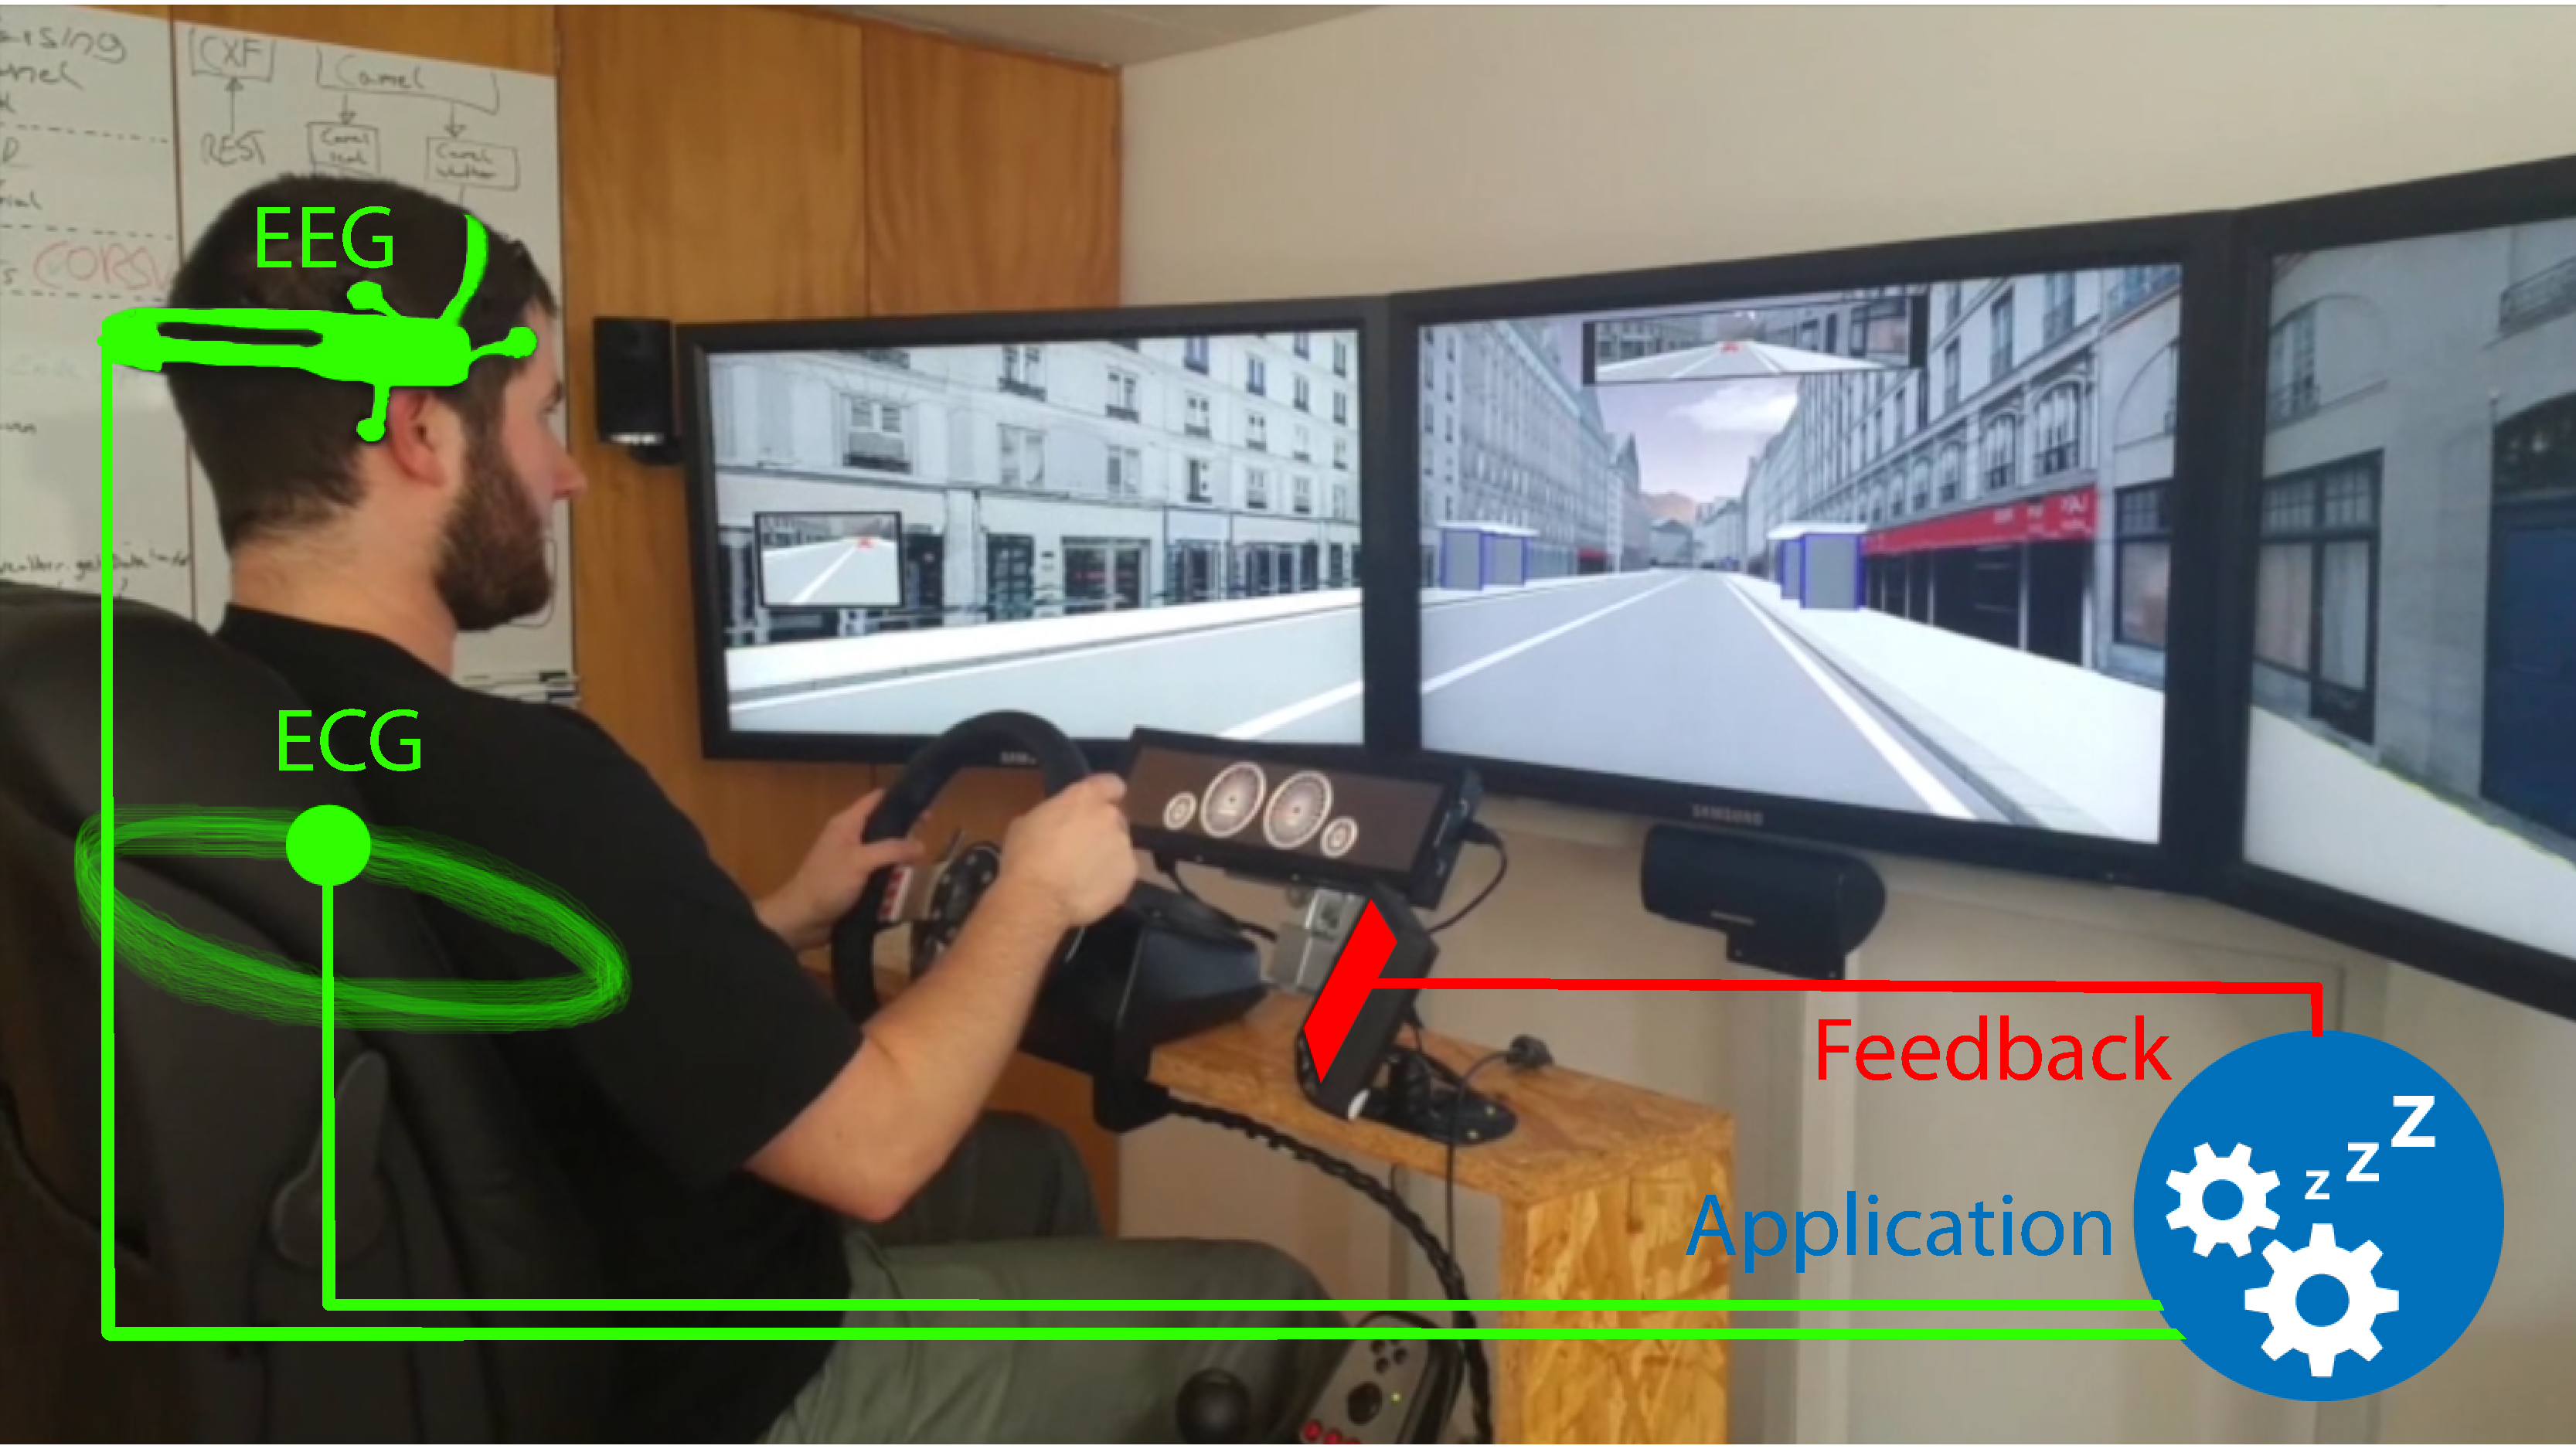
\includegraphics[width=\columnwidth]{aufbau}
    \caption[Skizze des Systemaufbaus]{Skizze des Systemaufbaus: Das EEG liefert Daten an die Applikation und ein Feedback-Device warnt den müden Fahrer. Bild zeigt den Fahrsimulator der \acl{RTU}. \label{fig:sketch}}
  \end{center}
\end{figure}

Zur Gruppe der Sicherheitsrelevanten \acl{FASs} gehört auch die \acl{ME}. Beispielsweise rät die \acl{ME} "`Attention Assist"' von Daimler dem Fahrer, zu gegebenem Anlass, eine Pause einzulegen und zeigt ein Kaffeesymbol im Cockpit an \cite{Daimler}. So wird müdigkeitsbedingte Unachtsamkeit oder Sekundenschlaf, die oftmals schwere Unfällen zur Folge haben, entgegengewirkt.

In Deutschland wurden 2015 rund 2,5 Mio. Unfälle polizeilich aufgenommen, die Zahl der Verkehrstoten liegt bei 3.450 \cite{accident_statistic}. Neben überhöhter Geschwindigkeit, zählt laut dem Deutschen Verkehrssicherheitsrat Müdigkeit zu den häufigsten Unfallursachen und ist damit für jeden fünften schweren Unfall verantwortlich \cite{dvr_statistic}. Dies verdeutlicht das Potential einer frühzeitigen Erkennung von Müdigkeit und einer Meldung an den Fahrer.

\problemDetail

Daraus ergeben sich Anforderungen für ein multimodales System zur \acl{ME}  (Abb. \ref{fig:sketch}). Es existieren bereit diverse Systeme, denen es jedoch oftmals an Komfort und Portabilität mangelt. Ziel dieser Arbeit ist die Entwicklung einer solchen Anwendung mit einem EEG-Headset. 
Dessen Signale werden verarbeitet und mit einem KNN klassifiziert, um den Fahrer rechtzeitig vor Übermüdung und deren Folgen zu warnen.
Statt einem klassischen EEG, wie es in der Medizin eingesetzt wird, wird ein EPOC Emotiv genutzt, dadurch soll die Beeinträchtigung des Fahrers verringert werden. Auch wenn sich selbst dieser Ansatz weniger für den Serienbetrieb eignet, wird das Handling deutlich verbessert. So kann das gesamte System beispielsweise für die Validierung von berührungslosen Systemen (bspw. Kamerabasiert) verwendet werden. Das ganze System soll leicht portierbar sein, um es in einem echten Fahrzeug testen zu können. Jedoch werden die notwendigen Testdaten im Rahmen des Projekts im Fahrsimulator der \acl{RTU} aufgenommen.

\tofc


\section{EEG Headset}
\label{chap:eeg}
Für das Projekt wurde ein EMOTIV Epoc+ EEG Headset \footnote{\url{http://emotiv.com/epoc}} (Abb \ref{fig:epoc_eeg}) verwendet. Es besitzt 14 EEG Kanäle, sowie ein Gyroskop und sendet seine Daten via Bluetooth an den Rechner. Das Headset wird über den Kopf gestülpt und besitzen an den Sensorenden einen Filz der mit Kochsalzlösung befeuchtet wird. 

\begin{figure}[h] 
  \begin{center}
    \includegraphics[width=0.75\columnwidth]{epoc_eeg}
    \caption[EMOTIV Epoc]{Das EMOTIV Epoc+ EEG Headset wird einfach über den Kopf gestülpt.\label{fig:epoc_eeg}}
  \end{center}
\end{figure}

Die Sensoren Anordnung ist an das internationale 10-20 System \cite{10-20}  angelehnt (\ref{fig:epoc_sensors}). Hierbei handelt es sich um eine standardisierte relative Anordnung der Elektroden. Die Rohdaten werden Abtastrate von 128 geliefert und enthalten neben dem Wert auch die Signalstärke (Qualität). Leider liefert die mitgelieferte SDK die Rohdaten nicht in Echtzeit, weshalb die Open-Source Lösung Emokit\footnote{\url{https://github.com/openyou/emokit}} eingebunden wurde.

\begin{figure}[h] 
  \begin{center}
    \includegraphics[width=0.5\columnwidth]{epoc_sensors}
    \caption[EEG Sensoren]{Die 14 Kanäle (Grün), sowie die beiden Qualitätssensoren (Gelb).\label{fig:epoc_sensors}}
  \end{center}
\end{figure}

\section{Stand der Technik}
\label{chap:state}
Systeme zur Erkennung von Müdigkeit versuchen mit verschiedenen Parametern herauszufinden, ob sich die Person (der Fahrer) noch in einem aufmerksamen Zustand befindet. Die lässt sich in drei Bereiche unterteilen: Fahrverhalten, Computer-Vision (CV) und Körpersensoren. Die beiden ersten Bereich werden nur für die manuelle Markierung von Datensätzen genutzt. Die folgenden Ansätze beziehen sich ausschließlich auf die Erkennung mit Körpersensoren.

Für die Erkennung von Müdigkeit werden verschiedene Körpersensoren bzw. deren Kombination (multimodal) eingesetzt. Meist werden elektrische Spannung am und im Körper gemessen. 
Neben dem EEG, werden bspw. die Elektrokardiographie (EKG) oder Elektrookulografie (EOG) genutzt. Beim EKG wird die elektrische Aktivität des Herzmuskels erfasst, um bspw. die  Herzfrequenz zu bestimmen. Das EOG misst die Bewegung der Augen, um bspw. Blinzeln zu erkennen.

Ansätze mit einem EKG allein, zeigten in verschiedenen Arbeiten kein eindeutiges Ergebnis \cite{Vicente_6164509}, \cite{Rogado_4913155}. Beide versuchten Informationen aus der Herzfrequenzvariabilität zu erhalten und diese zu klassifizieren.

Khushaba et al. \cite{Khushaba_5580017} versuchten EEG, EKG und EOG zu verbinden und verglichen verschiedenen Kombinationen. Mit einem "`fuzzy wavlet"' basierten Algorithmus wurde die Signale aufbereitet und zeigten, dass ein EEG alleine bereits ausreicht. Die Kombination eines EEG mit EKG bzw. EOG verbesserte das Ergebnis nicht signifikant. Auch Johnson et. al \cite{Johnson11} kamen zu der Erkenntnis, dass ein EEG ausreicht und das genutzte EOG nicht benötigt wird. 

\cite{Subasi:2005:ARA:1707423.1707550} konnten mit einem EEG die Zustände "`Wach"', "`Schläfrig"' und "`Schlafend"' unterscheiden. Die Wavelet-Transformation und das genutzte künstliche Neuronale Netz (KNN) führten zu einer Erkennungsrate von 93\%. Vuckovic et al. fanden den besten Algorithmus für die Initialisierung des KNNs: Der Learning Vector Quantization Algorithmus. Im Vergleich mit EEG-Experten erreichte das KNN eine Übereinstimmung von 90\%. Huang et al. \cite{Huang_548971} nutzten ein Hidden Markov Modell zu Erkennung und erreichten eine gute Erfolgsrate.
Lin et al. \cite{Lin05eeg-baseddrowsiness} nutzten die Unabhängige Komponenten Analyse (UKA) und Lineare Regression (LR) und konnten zeigen, dass hiermit  bis zu 88\% richtige Ergebnisse erzielt werden können. 

Die betrachteten Arbeiten unterstreichen die Eignung des EEGs um Müdigkeit zu erkennen. Kombiniert mit anderen Sensoren können die Ergebnisse nur noch leicht verbessert werden.


\section{Testdatenbeschaffung}
\label{chap:data}
Um Daten von übermüdeten Fahrern zu erhalten, kann natürlich kein Versuch im Straßenverkehr durchgeführt werden. Die Fremd- und Eigengefährdung wäre einfach zu groß. Darum fanden die Versuche in einer Simulationsumgebung statt. Für das Experiment wird im Fahrsimulator eine Nacht-Autobahnfahrt simuliert. Verschiedene Studien \cite{Engstrom_2322937}, \cite{Horne_1757738} legen nahe, dass sich  Simulationen zwar von der Realität unterscheiden, dass jedoch die Ergebnisse trotzdem valide und brauchbar sind.

Für den Versuch werden neben den rohen EEG Signalen, auch die Fahrzeugdaten, sowie die Simulation und der Fahrer aufgenommen. Weiterhin kann der Versuchsleiter auch Besonderheiten protokollieren (Abb. \ref{fig:experiment}).

\begin{figure}[h] 
  \begin{center}
    \includegraphics[width=\columnwidth]{experiment}
    \caption[Experiment]{Der Versuchsaufbau für die Erkennung von Müdigkeit mit den Datenströmen aus der Fahrerkabine zur Testüberwachung. \label{fig:experiment}}
  \end{center}
\end{figure}

Im Versuch sollte der Fahrer eindeutige Anzeichen von Müdigkeit zeigen. Dies kann durch verschiedene Versuchsparameter begünstigt werden. So zeigt eine Studie, dass Unfälle meist zwischen 2:00 - 6:00, sowie 14:00 - 16:00 Uhr passieren \cite{Horne_1757738}. Auch die Schlafmenge von weniger als 6 Stunden in der Nacht vor dem Experiment erhöht die Chance auf Anzeichen \cite{Engstrom_2322937}. Das Geschlecht oder Alter der Probanden ist nicht relevant. Vor dem Experiment sollten jedoch keine Drogen, Alkohol oder Kaffee eingenommen werden. Ein Führerschein ist von Vorteil, aber nicht zwingend notwendig.

Auch die Teststrecke (Abb. \ref{fig:drivingtask}) trägt zur Erhöhung der Müdigkeit bei. Monotone Autobahnfahrten die größtenteils geradeaus verlaufen, ohne andere Verkehrsteilnehmer und konstanter Geschwindigkeit führen eher zu einer Übermüdung. Nach diesen Kriterien wurde eine endlose zweispurige Autobahnkarte mit einer Geschwindigkeit von konstant 130Kmh erstellt. Sie spielt zudem Nachts und ist eher Dunkel gehalten, was besonders anstrengend für die Augen ist.

\begin{figure}[h] 
  \begin{center}
    \includegraphics[width=0.75\columnwidth]{drivingtask}
    \caption[Driving Task]{Die Autobahnkarte für den Versuch verläuft endlos geradeaus, Nachts und bei konstanter Geschwindigkeit. \label{fig:drivingtask}}
  \end{center}
\end{figure}

Für einen Versuch werden 40 Minuten angesetzt. Fünf Minuten werden für eine kurze Einführung, 30 Minuten für die Testfahrt und wieder fünf Minuten für eine kurze Einschätzung mit Fragebogen.

Anhand der aufgenommenen Daten werden nun Stellen gesucht, an denen die Testperson eindeutige Anzeichen von Müdigkeit zeigt. Eindeutig sind Verhaltensweisen wie häufiges Gähnen und Einnicken (Kopf fällt nach vorn) - Diese Merkmale werden häufig in CV-Ansätzen genutzt. 
Auch Verhaltensmerkmale wie, von der Spur abkommen und heftig Gegenlenken oder deutliche Veränderungen der Geschwindigkeit können Anzeichen für eine Unachtsamkeit wegen Müdigkeit sein.
Diese Stellen werden dann in den EEG Daten mit dem Label "`Müde"' markiert, alle anderen mit "`Wach"'. Die EEG Sequenzen können dann auf eindeutige Varianzen untersucht werden. Im nächsten Kapitel ist dies Thema der  Datenaufbereitung.


\section{PoSDBoS - Müdigkeitserkennung mit EEG-Headset}
\label{chap:implementation}

Abbildung \ref{fig:data_stream} zeigt die Gesamtübersicht des entwickelten Systems dar. Alle blauen Klassen der Anwendung wurden in Python 2.7 implementiert. Der Fahrsimulator und seine Schnittstellen (rosa) in Java und C\#. Abschnitt \ref{sec:fetching} befasst sich mit den Rohdaten und deren Weiterreichung im System. Die Verarbeitung der Rohdaten ist Thema von Abschnitt \ref{sec:processing}. Im folgenden Abschnitt werden daraus die passenden Merkmale extrahiert. In Abschnitt \ref{sec:classification} wird die Arbeitsweise des Klassifikators näher beleuchtet. 


\begin{figure*} 
  \begin{center}
    \includegraphics[width=12cm]{data_stream}
    \caption[Aufbau]{Das entwickelte System zur Müdigkeitserkennung. \label{fig:data_stream}}
  \end{center}
\end{figure*}

\subsection{Datensammlung}
\label{sec:fetching}
 
Das EEG Headset schickt enkodierte Byte-Sequenzen via Bluetooth, an die proprietären Emotiv Premium Libraries oder die Open-Source Lösung Emotkit (vgl. \ref{chap:eeg}). Die Emokit Klasse wurde für das Projekt leicht modifiziert, sodass sie sich ins System einfügt. So wurde Unterstützung für das neueste EPOC+ Modelle implementiert, sowie die Möglichkeit, Testdaten  aus aus dem TableReader zu versenden. 
Die dekodierten Rohdaten enthalten 14 EEG Kanäle mit Wert und Qualität, die Gyroskopwerte in X- und Y-Richtung und einen Zeitstempel (Abb. \ref{fig:data_processing}). Diese Daten können als CSV gespeichert werden, sowie an einen HTTP-Server oder direkt an den DataCollector übergeben werden. Über den Server integriert die SimToCAN Anwendung via HTTP die EEG Daten in den Fahrsimulator und das virtuelle Steuergerät (\ref{chap:data}).

\begin{figure}[h] 
  \begin{center}
    \includegraphics[width=5.5cm]{data_processing}
    \caption[Datenverarbeitung]{Die Daten werden immer weiter reduziert und verarbeitet. \label{fig:data_processing}}
  \end{center}
\end{figure}

Der DataCollector kann Daten direkt oder aus einem HTTP-Client empfangen. Die Schnittstelle zum Fahrsimulator bzw. zum CAR-Interface ist vorbereitet. So ist es möglich die Datensammlung und die Datenverarbeitung auf verschiedenen Rechnern durchzuführen.

Die Aufgabe der DataCollector-Klasse ist es, die einzelnen Signale in Sequenzfenstern von 128 Signalwerten zu aggregieren. Das ist die Abtastrate des EEG-Headsets und entspricht somit in etwa den Signalen einer Sekunde. Es sind zwei dieser Fenster implementiert und sie überschneiden sich in der Hälfte. So ist gewährleistet, dass signifikante Stellen nicht verloren gehen. Die Fensterfunktion ist ein simples Rechteck, sodass alle Werte gleich gewichtet werden. Eine andere Fensterfunktion bspw. mit Glockenkurvenerlauf (Hamming- oder Hann-Fenster) wäre einfach einzubauen. Zudem fügt der DataCollector nur konfigurierte Kanäle hinzu, sodass sich die Datenmenge reduziert. Im folgenden Abschnitt werden die gefilterten Sequenzfenster nun verarbeitet und aufbereitet.


\subsection{Datenverarbeitung}
\label{sec:processing}
Die Signalsequenzen durchlaufen eine Verarbeitungskette (Abb. \ref{fig:data_processing_chain}) mit den Schritten Bandpassfilterung, Artefaktentfernung, Normalisierung, Fouriertransformation und Aufteilung nach Frequenzbändern.

\begin{figure}[h] 
  \begin{center}
    \includegraphics[width=5.5cm]{data_processing_chain}
    \caption[Verarbeitungskette]{Die Signalsequenzen durchlaufen eine Verarbeitungskette \label{fig:data_processing_chain}}
  \end{center}
\end{figure}

Um Störungen zu eliminieren wurde das Signal zu Beginn außerhalb des Bereichs von 0.53Hz - 50Hz eliminiert. Dies war eine Empfehlung aus einer Antwort auf ResearchGate \cite{resGate} und zeigt bei Tests gute Ergebnisse. Der Bandpassfilter zentrierte das Signal zudem. 

Für die Anwendung wurde hierfür ein Buttworth-Filter\cite{Butterworth30} eingesetzt. Gleichung \ref{eq:butterworth} zeigt die Übertragungsfunktion mit $A_0$: Gleichspannungsverstärkung, $\Omega = \frac{f}{f_g}$: auf Grundfrequenz normierte Frequenz und $n$: Ordnung des Filters. Abbildung \ref{fig:butterworth_filter} zeigt exemplarisch Filterfunktionen verschiedener Ordnung mit den Grenzen von 500 bis 1250Hz. Alle Frequenzen darunter und darüber werden deutlich abgeschwächt bzw. gehen gegen null. Der Butterworth-Filter verläuft nahe Eins im gewünschten Bereich, fällt an den Grenzen ab und stellt sicher, dass das Signal an den Grenzen um $\frac{1}{\sqrt{2}} \approx 0.7071$ gemindert wird. Je höher die Ordnung, desto steiler geht die Funktion durch die angegebenen Grenzen. Der Filter lässt sich gut in Hardware realisieren.

\begin{equation} \label{eq:butterworth}
\left|\underline{A}\right|^2 = \frac{A_0^2}{1+ k_{2n} \Omega ^{2n}}
\end{equation}

\begin{figure}[h] 
  \begin{center}
    \includegraphics[width=5.5cm]{butterworth_filter}
    \caption[Butterworth-Filter]{Die Filterfunktion eines Butterworthfilters 2., 4,. und 8. Ordnung im Frequenzbereich von 500 bis 1250Hz. \label{fig:butterworth_filter}}
  \end{center}
\end{figure}

Bei der Analyse der Histogramme der Signalwerte, zeigte sich eine Häufung der Amplituden im Bereich von -100 bis 100 (siehe Abb. \ref{fig:raw_histo}). Außerhalb dieses Bereichs wurde als Artefakte angesehen und herausgefiltert (als ungültig markiert).

\begin{figure}[h] 
  \begin{center}
    \includegraphics[width=\docwidth]{raw_histo}
    \caption[Rohsignal und Histogramm]{Die Rohsignale pro Sensore und das dazugehörige Histogramm. Die Werte verteilen sich zwischen -8000 bis 8000, ein deutliches Maximum im Histogramm ist zwischen -100 und 100 erkennbar.  \label{fig:raw_histo}}
  \end{center}
\end{figure}

Die gefilterten Signal werden dann auf einen Bereich von -1 bis 1 normalisiert, dazu werden die Signale durch den jeweiligen Maximalwert bzw. Betrag des Minimalwertes geteilt (In diesem Fall 100). Dieses Vorgehen stellt sicher, dass die absolute Amplitude keinen Einfluss auf die Gewichtung im Klassifikator hat. Zudem wird die Datenmenge wiederum reduziert. Im letzten Schritt werden die Signale in ihre Frequenzbänder (EEG-Bänder) unterteilt. Hierzu werden die Signale in ihr Frequenzspektrum zerlegt und bestimmte Frequenzbereiche extrahiert. Diese EEG-Bänder gliedern sich in folgende Frequenzbereiche und werden nach griechischen Buchstaben benannt:
\begin{itemize}
 \item $\delta$ : 0,1 bis < 4Hz
 \item $\theta$ :   4 bis < 8Hz
 \item $\alpha$ :   8 bis < 13Hz
 \item $\beta$  :  13 bis < 30Hz
 \item $\gamma$ :  > 30Hz
\end{itemize}
Die Frequenzbereiche sind nicht einheitlich definiert und variieren unter Umständen. Die Frequenzbereich sind aus Empfehlungen der IFCN entnommen \cite{ifcn}. Den Frequenzbändern werden verschiedene Eigenschaften zugesprochen \cite{lei2011,Lv2010,Gundel1992}. Delta Wellen treten bei Erwachsenen häufig in der traumlosen Tiefschlafphase auf. Theta-Wellen zeigen sich bei Schläfrigkeit und leichtem Schlaf. Mit leichter Entspannung und entspannter Wachheit (mit geschlossenen Augen) werden Alpha-Wellen assoziiert. Beta Wellen treten während der REM-Schlafphase oder unter Einwirkung von Psychopharmaka auf. Gamma-Wellen gehen häufig mit starker Konzentration oder Meditation einher.

Um die einzelnen Frequenzbänder zu erhalten wird eine Fast-Fourier-Transformation \cite{Bochner_1} durchgeführt. Alternativ wäre auch ein Wavelet-Transformation \cite{Chui:1992:IW:163196} möglich gewesen. Beide Ansätze fanden sich in der Literatur Recherche, aus Zeitgründen wurde auf einen Vergleich der Ansätze verzichtet. 
Die Fourier-Transformation bildet ein zeitdiskretes endliches Signal, auf ein diskretes, periodisches Frequenzspektrum ab (siehe Abb. \ref{fig:fft_example}). Um die Frequenzbänder zu erhalten, wird das Ergebnis auf die gewünschten Frequenzen reduziert.

\begin{figure}[h] 
  \begin{center}
    \includegraphics[width=\docwidth]{fft_example}
    \caption[Fast Fourier Transformation]{Oben: EEG Signal darunter das Frequenzspektrum. Unten: die selbe Anordnung nur für ein Tonsignal, das Tonsignal schwingt mit 12KHz, dies zeigt sich durch ein Maximum bei dieser Frequenz. \label{fig:fft_example}}
  \end{center}
\end{figure}


\subsection{Mermalsextraktion}
\label{sec:extraction}
\textbf{TODO}

\subsection{Klassifikator}
\label{sec:classification}
Nachdem in vorherigen Abschnitt eine passende Merkmalsmenge erstellt wurde, geht es nun um die Entscheidung, ob der Fahrer Müde oder Wach ist bzw. ob das System eine Müdigkeitsmeldung erscheinen lässt. Für diese Klassifizierung werden im allgemeinen Machine-Learning-Algorithmen verwendet. Anhand von markierten Datensätzen wird versucht den Algorithmus zu Trainieren (Überwachtes Lernen). Dies dient dem Ziel, dass er auch unbekannte Daten klassifizieren kann. Dieser Vorgang wird Generalisierung bezeichnet und ist auch im menschlichen Lernen ein wichtiger Schritt.

Für die Anwendung wurde zur Klassifizierung ein künstliches Neuronales Netz (KNN) ausgewählt. Es basiert auf einem erweiterten Perceptron / McCulloch-Pitts-Neuron \cite{ann} und ist der Funktionsweise des menschlichen Gehirns bzw. seinen Neuronen nachempfunden\cite{marsland_opac-b1129336}. Ein KNN lässt sich im einfachste Fall durch eine Merkmalsmenge $X = x_1, x_2 ... x_n$, dazugehörige Gewichte $W = w_1, w_2 ... w_n$, eine Übertragungsfunktion $\sum$ und eine Schwellwertfunktion $\theta$ beschreiben (Abb. \ref{fig:perceptron}).

\begin{figure}[h] 
  \begin{center}
    \includegraphics[width=5.5cm]{perceptron}
    \caption[Schema eines Perceptrons / McCulloch-Pitts-Neurons]{Darstellung eines McCulloch-Pitts-Neurons. Die Merkmale $X$ werden mit den Gewichten $W$ multiplziert und in $\sum$ summiert. Wenn $h > \theta$ "`feuert"' das Neuron ($o = 1$) \cite{marsland_opac-b1129336}. \label{fig:perceptron}}
  \end{center}
\end{figure}

Dieser Aufbau kann schon einfach Aufgaben, wie bspw. ein logisches "`UND"', lösen. Jedoch lässt sich schon ein logisches "`XOR"' nicht mehr abbilden. Dafür müssen weitere Schichten von Neuronen (Hidden Layers) hintereinander geschaltet werden - das sog. Multi Layer Perceptron (MPL, Abb. \ref{fig:mlp}).

\begin{figure}[h] 
  \begin{center}
    \includegraphics[width=5.5cm]{mlp}
    \caption[Schema eines Multi-Layer-Perceptrons]{Darstellung eines Neuronalen Netzes mit mehreren Schichten (Multi Layer Perceptron, MLP)\cite{marsland_opac-b1129336}. \label{fig:mlp}}
  \end{center}
\end{figure}

Es exisitiert kein bekannter Algorithmus für die Wahl der optimalen initialen Parameter eines KNNs. Vuckovic et al. \cite{Vuckovic2002349} hatten sich mit diesem Thema genauer beschäftigt und die Ergebnisse werden für die Versuche herangezogen.
\textbf{TODO}


\section{Ergebnis}
\label{chap:result}
\textbf{TODO}
Da das EEG in den letzte 4 Monaten in Reparatur und somit nicht verfügbar war, sind die Ergebnisse bisher nicht aussagekräftig. Weder das Experiment, noch die Merkmalsextraktion und die Klassifizierung konnten sinnvoll evaluiert werden. 

Teil eins (1-4) der Anforderungen (vgl. Tab \ref{tab:requirements}) kann erst nach erfolgreicher Implementierung getestet werden. Die Portierung ist theoretisch sehr einfach möglich, wenn während der Fahrt ein Laptop genutzt wird (5). Die Handhabung und Komfort des Headsets ist im Vergleich zu medizinischen EEGs deutlich verbessert (6). Das EEG lässt sich ähnlich wie eine Mütze tragen und ist sehr leicht, sodass man schnell vergisst, dass es da ist. Die kabellose Übertragung sorgt für maximale Beweglichkeit. Wie schon angenommen, ist es jedoch für den Produktiveinsatz ungeeignet.

Tests auf einem Smartphone oder Tablet müssen gesondert erfolgen, da es unter anderem von den Treibern des EEG Headsets abhängt (7). Auch Lasttests sind erst nach fertiger Implementierung wirklich aussagekräftig (8). Der Einbau in die Simulationsumgebung ist bis zum eintragen der Werte im CAN-Bus umgesetzt. Das Herausnehmen der Werte ist noch nicht vollständig umgesetzt, da bisher die Integration der CarInterface Anwendung nicht funktionierte (9). Die PoSDBoS Anwendung lässt sich sehr gut auf verteilten Systemen ausführen, auch über den Anwendungsfall des Fahrsimulators hinaus. Die akquirierten Daten können via http an die Verarbeitungsschicht übertragen werden. Auch das Verschicken des Ergebnisses der Klassifizierung per http wäre denkbar und einfach umzusetzen (10). Die Art der Benachrichtigung über eine erkannte Müdigkeit ist derzeit noch nicht vollständig umgesetzt. Dem Fahrer wird entweder ein grüner oder roter Bildschirm angezeigt. Ob dies die passende Form ist, bleibt zu klären.

Die komplette Anwendung ist mit Docstring\footnote{\url{https://www.python.org/dev/peps/pep-0257/\#what-is-a-docstring}} versehen, aus denen eine html-Dokumentation erzeugt werden kann. Weiterhin sind schwierige Code-Teile mit einfachen Beispielen erweitert, um den Einstieg zu erleichtern. Ob es so möglich ist, als Neuling, selbständig die Anwendung zu verstehen bzw. zu erweitern hängt wohl auch von der jeweiligen Person ab. Werden jedoch Veränderungen vorgenommen, kann durch die Unit-Tests sichergestellt werden, dass die Klassen weiterhin das Richtige tun. Integrationstests wären eine sinnvolle  Erweiterung.


\section{Fazit und Ausblick}
\label{chap:conclusion}
Die Ergebnisse zeigen eine vielversprechende Grundlage und bilden das Grundgerüst für weitere Arbeiten. Die passende Architektur und Infrastruktur ist vorbereitet. Die Annahmen der Experiment-Hypthese wurde bestätigt, wenngleich sie sich nicht im erwarteten Maße in den EEG Daten niedergeschlagen hatte.

Die unzureichende Genauigkeit ist der wichtigste Anhaltspunkt der weiteren Forschung. Es werden derzeit lediglich zwei von drei Sequenzen aus den besten Daten richtig erkannt. 
Die Gründe hierfür lassen sich nicht eindeutig klären. Es könnte bei der Datenaquise - dem Experiment - beginnen, an Fehlern oder falscher Berechnungen während der Verarbeitung oder ungünstigen Startparametern beim Training des KNN liegen. Das Experiment hatte, bei Betrachtung objektiver Merkmale, sowie subjektiver Einschätzung der Testpersonen selbst, den gewünschten Effekt. Für weitere Schritte könnten die Experimente wiederholt werden und ggf. über einen längeren Zeitraum (\textasciitilde 1h) laufen. So wäre der Unterschied zwischen Wach und Müde unter Umständen deutlicher erkennbar. Auch die Aufnahme von Testdaten in verschiedenen Szenarien (Abwechslungsreiche Tagfahrt und langweilige Nachtfahrt) und unterschiedlichen Startparametern (bspw. Schlafmenge vor dem Experiment), könnten die Veränderung deutlicher machen.
Um Fehler beim Headset und den gelieferten Daten auszuschließen, 
müssen zuvor allerdings die Daten des Headsets und der genutzten Emokit Bibliothek noch einmal validiert werden.
Die Berechnungen Verarbeitungskette könnten mit etablierte EEG-Bibliotheken verglichen und werden. 



\balance
\bibliographystyle{unsrt} % abbrv, alpha, plain, unsrt, apalike
\bibliography{Kapitel/Literatur}


\end{document}
